
%preamble

\documentclass[14pt]{article}
\usepackage{graphicx}
\graphicspath{ {./images/} } 
\usepackage[utf8]{inputenc}
\usepackage{latexsym}
\usepackage{url}
\usepackage{hyperref}
\usepackage{amsmath}
\usepackage{algorithm}
\usepackage{algorithmic}
\usepackage{enumitem,amssymb}
\usepackage{txfonts}
\usepackage{xcolor}

\begin{document}

\title{\Huge \textbf {Determinarea arborelui}\\
\textbf{de acoperire minim\u a}\\
(minimum spanning tree)}

\date{\Large\today}
\maketitle

\begin{center}

\vspace{20 mm}

\author{\huge Student: Neagoe Filip}

\vspace{10 mm}

\title{\huge Grupa: 1.2 B, anul I}
 
\vspace{10 mm}

\title{\huge\ Specializarea: CTI rom\^an\u{a}}
\maketitle

\newpage

\end{center}

\tableofcontents

\newpage

\title\textbf{-Rezumat-}

\vspace{3mm}

\large   \^In raportul urm\u{a}tor sunt prezentate dou\u{a} abord\u{a}ri ale algoritmilor Kruskal, respectiv Prim responsabili pentru determinarea arborelui de acoperire minim\u{a} a unui graf neorientat conex.
    
\maketitle

\section{\underline{Problema 4 - Arbori de acoperire minim\u{a}}}
\vspace{7mm}

\subsection{Enun\c tul problemei}
\vspace{2.5 mm}

S\u{a} se implementeze doi algoritmi diferiti care
determina arborele de acoperire minim\u{a} al unui graf neorientat conex dat.\\
\textbf{Sugestii}: doi dintre algoritmii Boruvka, Prim  ̧si Kruskal.

\vspace{2 mm}

\subsection{Algoritmii propu\c si}
\vspace{5mm}

\large{\underline{Algoritmul lui Prim}}
\vspace{4mm}

\begin{figure}[h]
\begin{center}
\begin{tabbing}
\textbf{PRIM}($a\_graph[ ][ ]$,$no\_of\_nodes2$)\\
1. \indent{\bf for} \=$i = 0$, $no\_of\_nodes$ {\bf do} \\
2. \indent            \> $k[i] = INT\_MAX$ \\
3. \indent            \> $min\_span\_tree = 0$ \\
4. $k[0] = 0$ \\
5. $ascendent[0] = -1$ \\
6. \indent{\bf for} \=$counting = 0$, $no\_of\_nodes2 - 1$ {\bf do} \\
7. \indent            \> $m = minimum\_key (k, min\_span\_tree, no\_of\_nodes2)$\\
8. \indent            \> $min\_span\_tree[m] = 1$ \\
9. \indent{\bf for} \=$n = 0$, $no\_of\_nodes2$ {\bf do} \\
10.\indent            \>{\bf if} \=$a\_graph[m][n]$  and  $min\_span\_tree[n]  ==  0$  and $a\_graph[m][n] < k[n]$ {\bf then} \\
11. \indent           \>           \> $ascendent[n]=m$ \\
12. \indent           \>           \> $k[n] = a\_graph[m][n]$\\
13. \indent{\bf for} \=$i = 1$, $no\_of\_nodes2$ {\bf do} \\
14. \indent            \> $\rhd$ print($ascendent[i]$,$i$,$a\_graph[i][$ascendent[i]$])$ \\
15.\indent             \> $\rhd$ print newline()\\
16.  \textbf{end} PRIM
\vspace{2mm}

\end{tabbing}
\caption{\colorbox{black}{\textcolor{white}{Pseudocod algoritm Prim}}}
\end{center}
\end{figure}

\vspace{20mm}

\newpage

\large{\underline{Algoritmul lui Kruskal}}

\vspace{10mm}
\begin{figure}[h]
\begin{center}
\begin{tabbing}
\textbf{KRUSKAL}($n$, $m$, $L[]$, $graph *G$)\\
$n = G -> no\_of\_vertices$\\
1. \indent{\bf for} \=$i = 0$, $m$ {\bf do} \\
2.    \indent{\bf for}    \=$j = i + 1$, $m$ {\bf do} \\
3.\indent            \>{\bf if} \=$G -> eEdge[ i ].weight  >  G -> eEdge[ j].weight$ {\bf then} \\
4. \indent                \>         \> $edge\ aux$ \\
5. \indent                \>         \> $aux = G -> eEdge[ i ]$ \\
6. \indent                \>         \> $G -> eEdge[ i ] = G -> eEdge[ j ]$ \\
7. \indent                \>         \> $G -> eEdge[ j ] = aux$ \\
8. \indent{\bf for} \=$i = 0$, $n$ {\bf do} \\
9. \indent            \> $L[i] = i$ \\
10.\indent  print newline()\\
11.\indent  print("MST are urmatoarele muchii: )\\
12.\indent  print newline()\\
13. \indent     \>{\bf while} \=$k < n - 1${\bf do} \\
14.\indent          \>{\bf if}    \=$L[G -> eEdge[ i ].start\_point]  !=  L[G -> eEdge[ i ].end\_point]$ {\bf then}\\
15. \indent                      \>     \> $k++$ \\
16. \indent                      \>     \> $coverage\_cost  =  coverage\_cost  +  G -> eEdge[ i ].weight$ \\
17.\indent  print $(G -> eEdge[ i ].start\_point,  G -> eEdge[ i ].end\_point )$\\
18.\indent  print newline()\\
19.$x = L [G -> eEdge[ i ].end\_point]$\\	
20.$y = L [G -> eEdge[ i ].start\_point]$\\
21. \indent{\bf for} \=$j = 0$, $n$ {\bf do} \\
22.\indent            \>{\bf if} \=$L[ j ] == x$ {\bf then} \\
23. \indent           \>           \> $L[ j ] = y$ \\
24.i++\\
25.\indent print newline()\\
26.\indent print("Costul total al acoperirii minime  =   ", coverage\_cost)\\
27.\indent  print newline()\\
28.  \textbf{end} KRUSKAL

\vspace{20mm}

\end{tabbing}
\caption{\colorbox{black}{\textcolor{white}{Pseudocod algoritm Kruskal}}}
\end{center}
\end{figure}

\newpage

In continuare sunt analizate si comparate c\^ateva aspecte ce diferentiaz\u{a} cei doi algoritmi descrisi anterior in limbaj pseudocod(\textbf{Figure 1, Figure 2}).

\vspace{7mm}

\begin{center} 
\begin{tabular}{|l|l|}
\hline \multicolumn{2}{|c|}{\textbf{Diferente intre Prim's algorithm si Kruskal's algorithm}}\\
\hline
\textbf{\colorbox{black}{\textcolor{white}{Prim's}}} & \textbf{\colorbox{black}{\textcolor{white}{Kruskal's}}}\\
\hline
-construie\c ste arborele de acoperire\\ minim\u{a} pornind din oricare vertex & -\^incepe s\u{a} construiasc\u{a} arborele\\& de la  muchia cu cea mai mic\u{a}\\& greutate(valoare) \\ -arborele care se formeaz\u{a} pe parcurs\\ r\u{a}m\^ane \^intotdeauna conectat \\& -arborele care se formeaz\u{a} r\u{a}m\^ane \\& \^in cele mai multe cazuri neconectat \\  -algoritmul lui Prim este mai eficace\\ in cazul grafurilor dense,\\ cu un num\u{a}r mai mare de muchii & -algoritmul lui Kruskal este mai\\& eficient pentru grafurile "r\u{a}sfirate",\\& cu num\u{a}r de muchii mai mic \\ -complexitatea timpului de execu\c tie :\\ $O(\|V\|^2)$,  V - num\u{a}r noduri & -complexitatea timpului de execu\c tie :\\& $O(ElogV)$, unde :\\& V - num\u{a}r vertexuri, E - num\u{a}r muchii \\ -pentru implementarea utiliz\^and\\ adjacency matrix,\\ cerin\c tele de memorie sunt :\\ $O(v^2)$, \\unde v reprezint\u{a} num\u{a}rul de noduri &  -cerin\c te de memorie:\\& $O(n)$,  n - num\u{a}rul de noduri\\
\hline
\end{tabular} \end{center} 
\vspace{5mm}

Complexitatea de spa\c tiu\textbf {(space complexity)} corespunz\u{a}toare fiec\u{a}rui algoritm const\u{a} at\^ at \^in resursele auxiliare de spa\c tiu necesare pe durata execu\c tiei, c\^ at \c si \^in dimensiunea datelor de intrare.A\c sadar, complexitatea de spa\c tiu (de memorie) este interconectat\u{a} \c si dependent\u{a} de dimensiunea input-ului aferent algoritmului.\\
\\
Totu\c si, \^in cele mai multe dintre cazuri, vom determina complexitatea de memorie contoriz\^and spa\c tiul auxiliar (temporar) necesar variabilelor \c si constantelor implicate \^in algoritm.\\
\\
\underline{\^In cazul algoritmului lui Prim} (\^in implementarea de fa\c ta), este utilizat\u{a} o matrice p\u{a}tratic\u{a} pentru a descrie leg\u{a}turile care se stabilesc \^intre nodurile grafului.Dimensiunea matricei este dictat\u{a} de num\u{a}rul de noduri introdus de c\u{a}tre utilizator \^in vederea gener\u{a}rii grafului ; \^in spe\c t\u{a}, spa\c tiul ocupat de matrice este direct propor\c tional cu dimensiunea datelor introduse de utilizator.\\De aici rezult\u{a} ca vom avea o complexitate p\u{a}tratic\u{a} ($O(v^2)$) a memoriei utilizate(clasa de complexitate p\u{a}tratic\u{a}).\\

\^In cadrul algoritmului mai sunt utilizate c\^ateva variabile, \^ins\u{a} acestea sunt nesemnificative \^in raport cu memoria consumata de matricea de stocare.\\
\\
\underline{\^In cazul algoritmului lui Kruskal}, este utilizat un tablou unidimensional de octe\c ti cu dimensiunea direct propor\c tional\u{a} cu num\u{a}rul de noduri ale grafului, la care se adaug\u{a} de asemenea c\^ateva variabile de tip \^intreg, complexitatea de memorie fiind liniara( O(n) ).\\
\\


\textbf{Similitudini} intre cele doua abordari:
\vspace{5mm}
\\
-ambii algoritmi trebuie sa evite formarea buclelor(cercurilor) in cadrul grafului;\\
-in ambele implementari, numarul nodurilor vizitate este minim si fiecare nod este vizitat o singura data;\\
-ambii algoritmi fac parte din categoria algoritmilor \textbf{Greedy}.

\begin{center}
   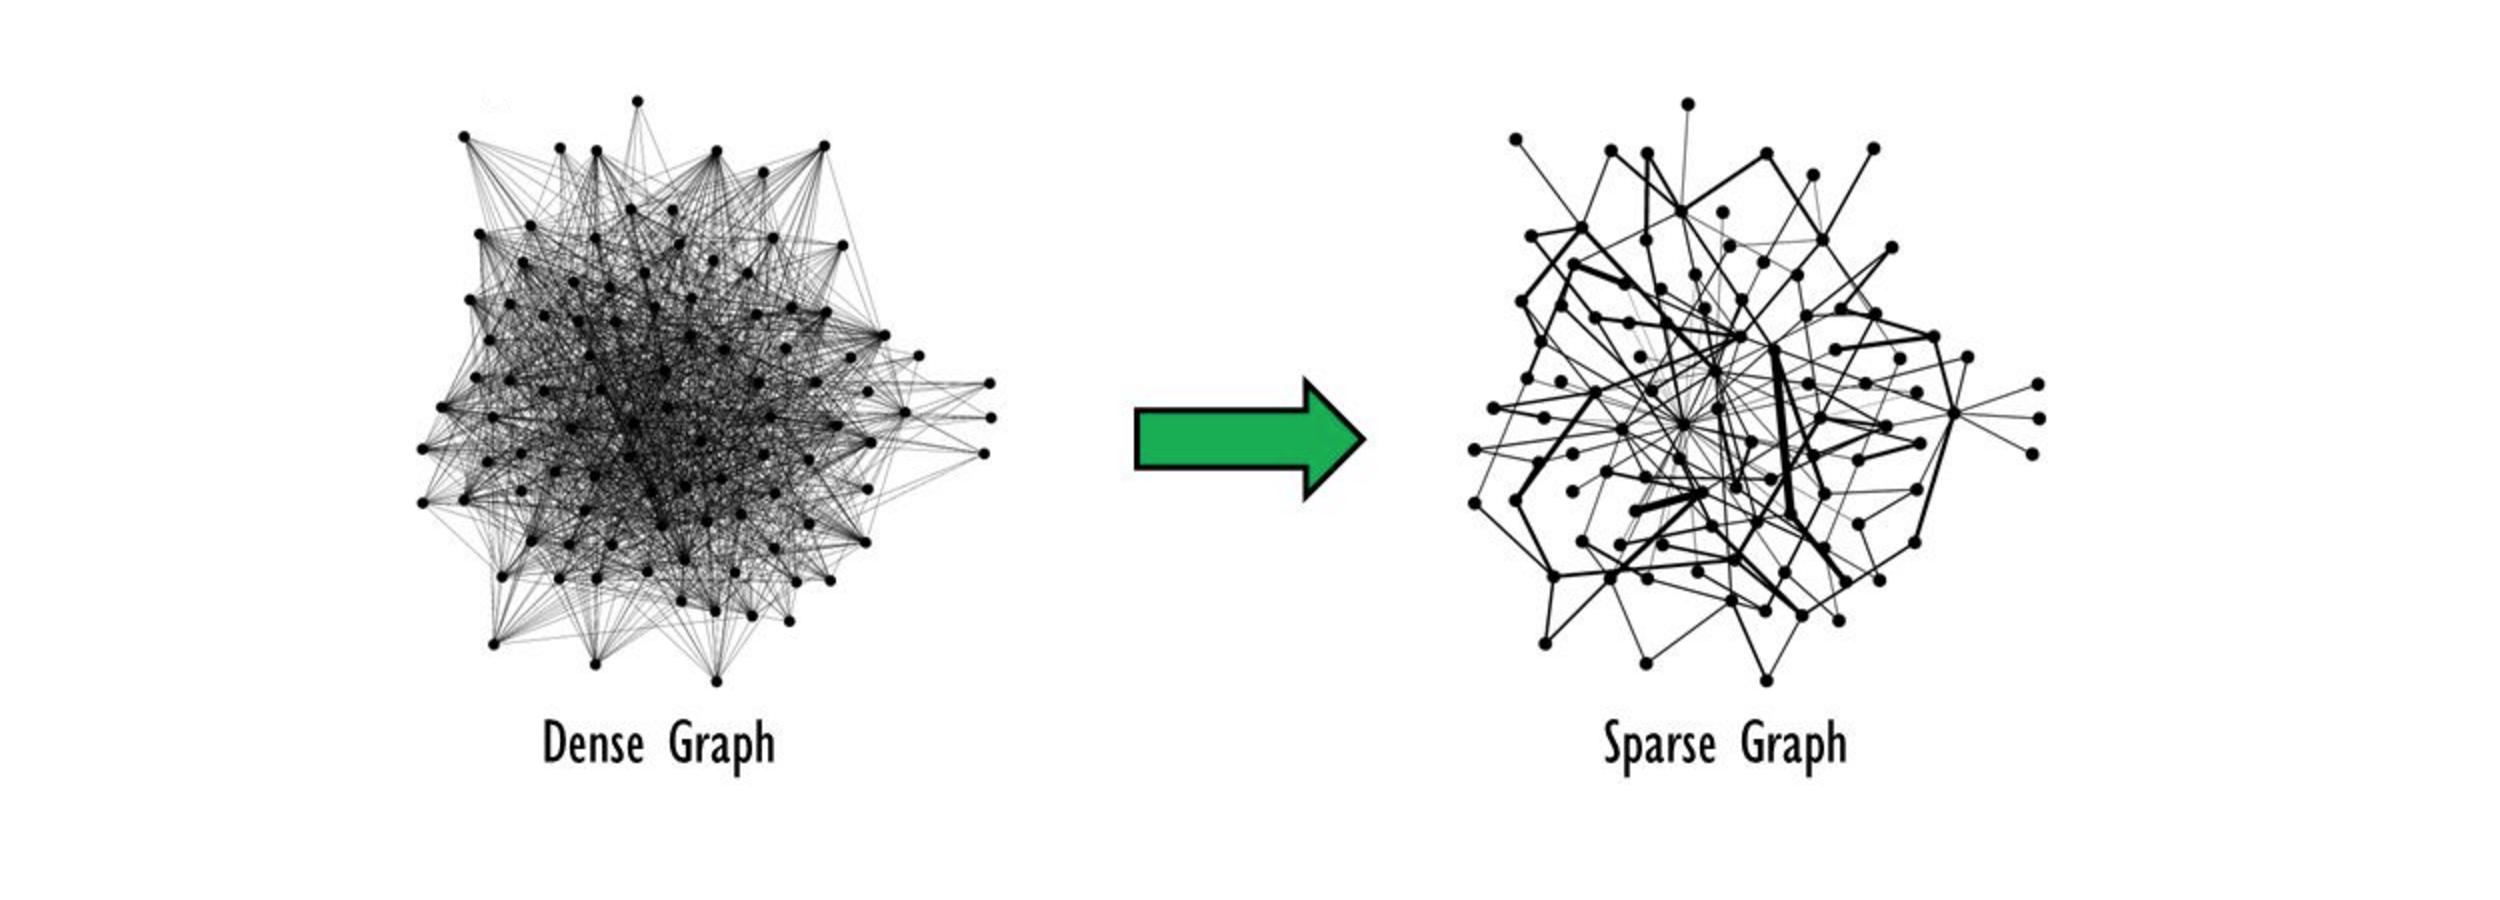
\includegraphics[width = 16cm, height = 10cm]{dense} 
\end{center}

\begin{center}
    \colorbox{black}{\textcolor{white}{ \textbf{-Graf dens vs graf r\u{a}sfirat(sparse)-}}} 
\end{center}

\^In imaginea urm\u{a}toare este eviden\c tiat\u{a} diferen\c ta dintre un arbore de acoperire si un arbore de acoperire \textbf{minim\u{a}}. 

\vspace{3mm}

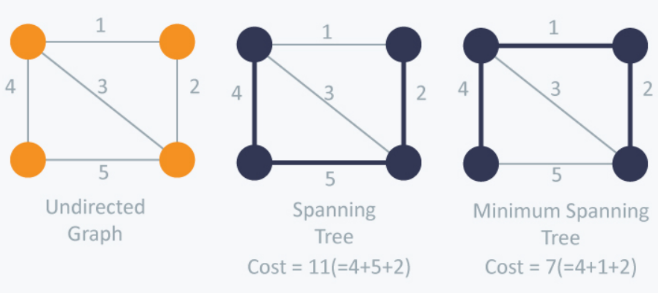
\includegraphics[width = 12cm, height = 5cm]{comparison}

\vspace{2mm}

\textbf{Observa\c tie:} pot exista mai multi arbori de acoperire, dar un \textbf{singur} arbore de acoperire minim\u{a} a unui graf.

\vspace{7mm}

\^In figura urm\u{a}toare este surprins\u{a} evolu\c tia construc\c tiei arborelui de acoperire minim\u{a} in cazul oper\u{a}rii \textbf{algorimului lui Prim} asupra grafului.
\\
\\
\\
\\


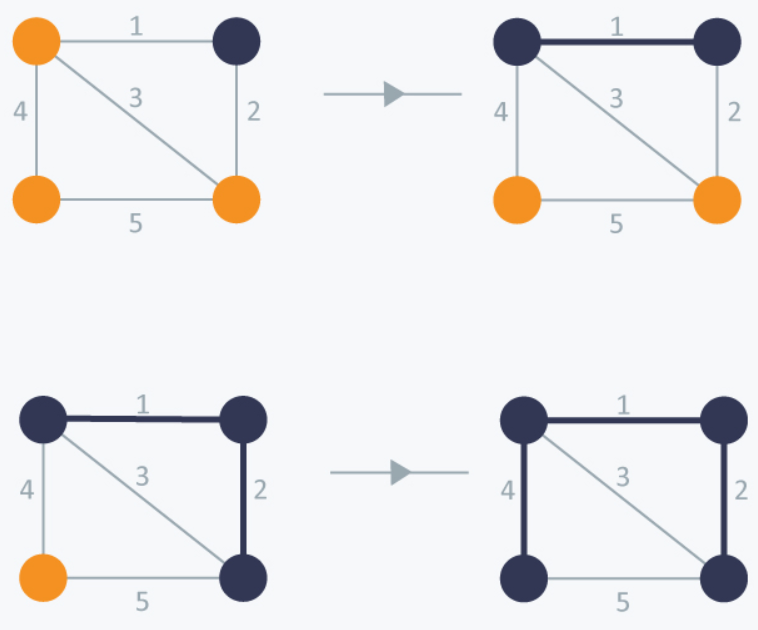
\includegraphics[width = 12cm, height = 12cm]{prim}

\newpage

Aceast\u{a} reprezentare surprinde modul de lucru al \textbf{algoritmului lui Kruskal} asupra unui graf conex, neorientat.

\vspace{10mm}

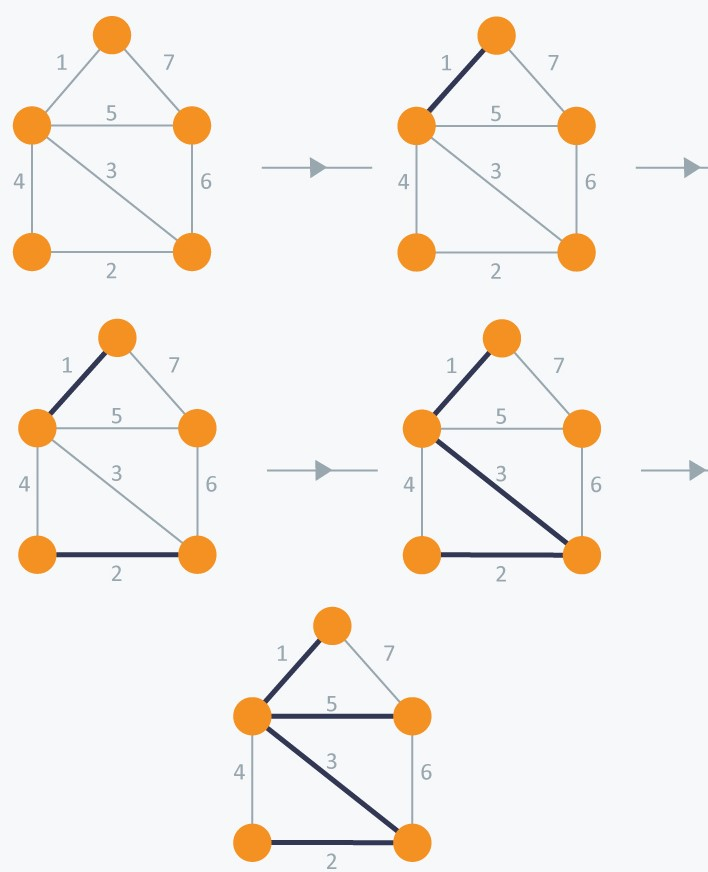
\includegraphics[width = 12cm, height = 12cm]{kruskal}

\vspace{10mm}

\^In continuare sunt ata\c sate doua link-uri la care pot fi vizualizate amina\c tii corespunz\u{a}toare celor 2 algoritmi:\\

\vspace{1mm}
-animatie algoritmul lui Prim :\\
\textcolor{blue}{\url{https://www.youtube.com/watch?v=wpV1wvHqyuY}}\\
-animatie algoritmul lui Kruskal :\\
\textcolor{blue}{\url{https://www.youtube.com/watch?v=o8Sqm1_3BRo}}

\newpage

\subsection{Datele experimentale}
\vspace{3mm}
\^In continuare este descris \^in limbaj pseudocod un algoritm responsabil pentru \textbf{generarea} unei matrice relevante pentru formarea ulterioar\u{a} a grafului(conform specifica\c tiilor impuse si necesare) pe care vor opera cei doi algoritmi, Prim, respectiv Kruskal.  

\vspace{5mm}
\begin{figure}[h]
\begin{center}
\begin{tabbing}

\large{\underline{Algoritm generator de date}}\\

\vspace{15mm}\\
\textbf{RANDOMIZE} ($adj\_matrix$, $no\_of\_nodes2$)\\
1.\indent print ("Introduceti numarul de noduri: ")\\
2.\indent read no\_of\_nodes2\\
3. \indent{\bf for} \=$i = 0$, $no\_of\_nodes2$ {\bf do} \\
4.   \indent{\bf for}     \=$j = 1$, $no\_of\_nodes2$ {\bf do} \\
5. \indent            \>{\bf if} \=$i = j$  {\bf then} \\
6. \indent               \>           \> $adj\_matrix[i][j] = 0$ \\
7. \indent            \>{\bf else} \\
8. \indent               \>           \> $adj\_matrix[ i ][ j ] = adj\_matrix[ j ][ i ] = randomize (1,10)$ \\
9. \indent{\bf for} \=$i = 0$, $no\_of\_nodes2$ {\bf do} \\
10. \indent{\bf for}     \=$j = 0$, $no\_of\_nodes2$ {\bf do} \\
11.\indent          \>           print $adj\_matrix[i][j]$\\
12.\indent print newline()\\
13. \textbf{end} RANDOMIZE

\vspace{20mm}

\end{tabbing}
\caption{\colorbox{black}{\textcolor{white}{Pseudocod generator date}}}
\end{center}
\end{figure}

\vspace{3mm}

\large\underline{{Descrierea algoritmului de generare a datelor}}
\vspace{3mm}

Algoritmul responsabil pentru generarea de date necesare test\u{a}rii algorimilor Prim si Kruskal (\textbf{Figure 3}) are drept scop principal generarea matricei adjencte (adjacency matrix) reprezentativ\u{a} pentru graful construit ulterior.\\

\^In functie de num\u{a}rul de noduri introdus de utilizator \^in vederea formarii grafului (\underline{linia 2}), programul genereaz\u{a} o matrice patratic\u{a} av\^and dimensiunea impus\u{a}.\\

Dup\u{a} introducerea num\u{a}rului de noduri, \^in urma itera\c tiei indicilor corespunz\u{a}tori liniilor, respectiv coloanelor matricei (\underline{linia 3}, respectiv \underline{linia 4}), se verific\u{a} egalitatea acestora (linia 5).Daca indicii se g\u{a}sesc a fi egali, elementul corespunz\u{a}tor pozi\c tiei descrise de ace\c stia este ini\c tializat cu valoarea "0" (\underline{linia 6}).\\

\^In cazul de fa\c ta, mul\c timea elementelor cu aceast\u{a} caracteristic\u{a} (\underline{i = j}) reprezint\u{a} diagonala principal\u{a} a matricei.\\

Contrar, elementele ai c\u{a}ror indici nu se confund\u{a} (nu sunt egali), se vor initializa cu valori generate aleatoriu ( apartin\^and intervalului setat de utilizator), precum si elementele cu pozi\c tii simetrice fata de acestea, raportate la diagonala principal\u{a} (\underline{linia 8} : elementele vor fi ini\c tializate cu valori aleatorii apar\c tinand intervalului [0, 10]).\\

Ulterior set\u{a}rii valorilor pentru elementele din componen\c ta matricei, se execut\u{a} afi\c sarea rezultatelor ob\c tinute in urma rul\u{a}rilor programului (\underline{liniile 9, 10, 11 s\c i 12}).\\

Algoritmul se \^incheie (\underline{linia 13}).\\

\vspace{2mm}

\textbf{Datele generate de acest algoritm}, \^in spe\c t\u{a}, matricea aferent\u{a} grafului, \textbf{sunt semnificative} pentru testele efectuate prin operarea algoritmilor Prim si Kruskal asupra lor deoarece respect\u{a} parametri si condi\c tiile impuse pentru o func\c tionare corespunz\u{a}toare.\\

Astfel, matricea generat\u{a} este in concordan\c t\u{a} cu formatul matricei unui graf neorientat, conex, ale c\u{a}rui muchii sunt populate cu valori generate in mod aleatoriu.De asemenea, elementele ai c\u{a}ror indici de pozi\c tie sunt egali (i = j) sunt i\c tilializa\c ti cu valoarea "0", fapt care indic\u{a} absen\c ta buclelor(self-loops) \^in graf.\\

Elementele simetrice fa\c t\u{a} de diagonala principal\u{a} au valori egale (pozitive) \^intruc\^at matricea corespunz\u{a}toare unui graf neorientat respect\u{a} aceast\u{a} condi\c tie si se \^incadreaza \^in acest tipar.

\newpage

\subsection{\large{Proiectarea experimental\u{a} a aplica\c tiei}}

\vspace{3mm}

\begin{itemize}

\item
%\begin{center}
\underline{\Large{Structura de nivel \^inalt a aplica\c tiei}}
%\end{center}
\vspace{10mm}

\begin{center}
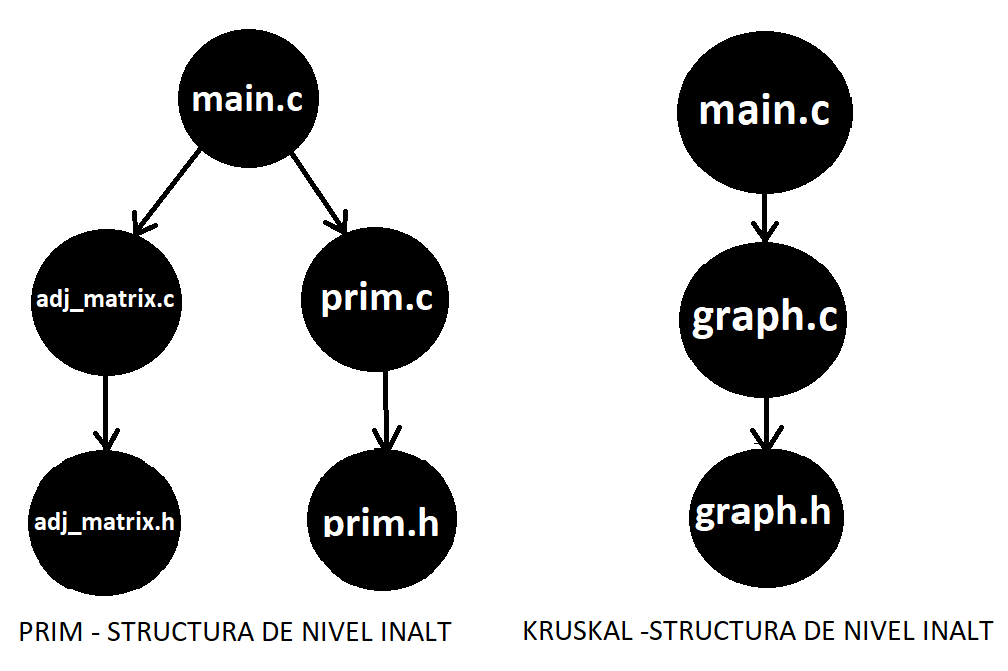
\includegraphics[width = 15cm, height = 10cm]{structuri.png}
\end{center}   

\vspace{3mm}

\footnote{Structurile de nivel \^inalt corespunz\u{a}toare celor doi algoritmi au fost realizate \^in programul Paint}

\vspace{1mm}
\item
\underline{\Large\textbf{{Descrierea mul\c timii datelor de intrare}}}
\vspace{2mm}

Este cunoscut num\u{a}rul de noduri ale grafului pe baza c\u{a}ruia se va genera matricea care descrie structura acestuia.Pe baza acesteia, cei doi algoritmi vor opera in vederea form\u{a}rii arborelui de acoperire minim\u{a}, respectiv, pentru calcularea costului s\u{a}u.
\newpage

\underline{\textbf{Tipul datelor de intrare :}}\\
\begin{itemize}
    \item 
    num\u{a}rul de noduri ale grafului - \^intreg
    \item
    matricea p\u{a}tratic\u{a} generat\u{a} aleatoriu - tablou bidimensional populat cu valori de tip unsigned int (valori \^intregi f\u{a}r\u{a} semn) 
\end{itemize}

Matricea generat\u{a} prin intermediul generatorului de date este stocat\u{a} \^intr-un fi\c sier de tip text de unde este accesata. 

\vspace{2mm}

\item
\underline{\Large\textbf{Descrierea iesirilor / rezultatelor}}

\vspace{3mm}

\^In urma execu\c tiei celor doi algoritmi se ob\c tine o list\u{a} a perechilor de noduri care alc\u{a}tuiesc arborele de acoperire minim\u{a} asociat grafului, \^insotite de valoarea corespunz\u{a}toare a acestora (costul muchiilor care conecteaz\u{a} nodurile respective).\\
\\
De asemenea, va fi returnat \c si rezultatul calculului costului total de acoperire minim\u{a} a arborelui asociat grafului, precum si timpii de execu\c tie ai algortimilor pentru fiecare set de date.  

\vspace{3mm}

\underline{\textbf{Tipul datelor de iesire / rezultatelor :}}
\vspace{2mm}

\begin{itemize}
    \item perechile de noduri - valori de tip \^intreg (int)
    \item costul total al acoperirii minime - valoare de tip unsigned int (\^intreg fara semn), \^intrucat costul aferent fiecarei muchii este pozitiv
    \item timpul necesar execut\u{a}rii programului pentru fiecare set de date (valoare de tip real)
\end{itemize}

\item
\underline{\Large\textbf{Lista tuturor modulelor aplica\c tiei \c si o scurt\c a descriere a lor}}

\vspace{1mm}

\begin{itemize}
    \item \textbf{Lista modulelor pentru aplica\c tia algoritmului lui Prim:}
    \\
    \begin{itemize}
        \item \textbf{main.c} - modulul principal al aplica\c tiei\\
    Acest modul este interconectat cu urm\u{a}toarele module ".c", iar func\c tionarea sa depinde de acestea.\\
    Main.c reprezint\u{a} modulul central care \^inglobeaza celelalte module ".c" al\u{a}turi de extensiile acestora.
        \item \textbf{adj\_matrix\_generator.c} - modulul responsabil de generarea matricei aferente grafului.
        \item \textbf{prim.c} - in cadrul acestui modul este elaborat algoritmul pentru prelucrarea grafului, \^in acest caz, algoritmul lui Prim.
        \item \textbf{adj\_matrix\_generator.h} - modul de tip header ata\c sat modulului sursa "adj\_matrix\_generator.c".\\
        Con\c tine prototipul func\c tiei "randomize" descrisa \^in  fi\c sierul surs\u{a} "adj\_matrix\_generator.c"
        \item \textbf{prim.h} - modul de tip header in care este specificat prototipul functiilor "minimum\_key", respectiv, "prim" descrise in fisierul sursa "prim.c".
        \\
    \end{itemize}
    
    
\item \textbf{Lista modulelor pentru aplica\c tia algoritmului lui Kruskal:}
\\
    \begin{itemize}
        \item \textbf{main.c} - modul principal al aplica\c tiei\\
        Spre deosebire de primul algoritm, \^in cazul algortimului de fa\c ta, \^in fisierul surs\u{a} "main.c" este descris algorimul lui Kruskal.\\
        De asemenea, acest modul apeleaz\u{a} alte module precum "graph.c".
        \item \textbf{graph.c} - modul surs\u{a} \^in care este descris modul de \^inc\u{a}rcare (generare) a grafului, de data aceasta, acesta fiind generat pe baza unui fi\c sier de tip text popular de c\u{a}tre utilizator.
        \item \textbf{graph.h} - modul de tip header corelat cu modulul surs\u{a} "graph.c" \^in care este specificat prototipul func\c tiei "create\_graph".
        Acest modul con\c tine si structurile ale unor elemente cu care se va opera(graf, muchie graf).
        \\
    \end{itemize}
    
    \item\textbf{Lista modulelor programului generator de date :}
    \\
    \begin{itemize}
        \item \textbf{main.c} - modulul principal al programului \c si unicul \^in acest caz.\^In cadrul s\u{a}u este descris\u{a} funct\c ia necesar\u{a} gener\u{a}rii matricei. 
        \\
    \end{itemize}
    \end{itemize}

    \item
  \underline{\Large\textbf{Descrierea procedurilor aplica\c tiei}}
    \vspace{1mm}
    \begin{itemize}
        \item \textbf{I )} \textbf{\underline{Algoritmul lui Prim}}
        \vspace{1mm}
      \begin{itemize}
           \item\underline{\textbf{modulul "adj\_matrix\_generator.c"}} \\
           \\
           \underline{\textbf{--func\c tia "randomize"--}} (\textbf{void} randomize)\\
           \\
           \textbf{-scop :} genereaza matricea aferenta grafului\\
           \textbf{-parametrii :}\\
                -\underline{$adj\_matrix[ ][ ]$} (tablou bidimensional de tip \^intreg)\\
                -\underline{no\_of\_nodes2} (parametru de tip \^intreg) ; semnific\u{a} num\u{a}rul de linii si de coloane ale viitoarei matrice.\\
           Func\c tia "randomize este de \textbf{tip void}. \^In consecin\c t\u{a}, nu are valoare de retur.
           \\
           \item \underline{\textbf{modulul "prim.c"}}\\
           \\
           \underline{\textbf{--func\c tia "minimum\_key--}} (\textbf{int} minimum\_key)\\
           \\
           \textbf{-scop :} g\u{a}se\c ste nodul din graf cu valoarea minim\u{a}, dintre nodurile neincluse \^inca in graf\\
            \textbf{-parametrii :}\\
            -\underline{k[ ]} (parametru de tip \^intreg) : \^in acest \c tablou unidimensional vor fi stocate valorile nodurilor la un moment dat, pentru a fi comparate ulterior.\\
            -\underline{min\_span\_tree[ ]} (tablou unidimensional de tip \^intreg) : contorizeaz\u{a} starea nodurilor, mai exact, dac\u{a} sunt sau nu incluse \^in arborele de acoperire minim\u{a}.
           -\underline{no\_of\_nodes2} (parametru de tip \^intreg) : se refer\u{a} la num\u{a}rul de noduri ale grafului.\\
           \textbf{-valoare de retur}\\
           -\underline{min} (valoare de tip \^intreg) : func\c tia returneaz\u{a} nodul de valoare minim\u{a}
           \\
           \\
            \underline{\textbf{--func\c tia "prim"--}}\\
            \\
            \textbf{-scop :} formarea arborelui unic de acoperire minim\u{a}\\
            \textbf{-parametri :}\\
            -\underline{a\_graph[][20]} (tablou bidimensional de tip intreg) : reprezint\u{a} matricea generat\u{a} aferent\u{a} grafului\\
            -\underline{no\_of\_nodes2} (parametru de tip \^intreg) : num\u{a}rul de noduri ale grafului\\
            \textbf{-valoare de retur}\\
            Func\c tia "prim" este de \textbf{tip void}, deci nu va returna nimic.
            \\
            \\
             \item \underline{\textbf{modulul "main.c"}}\\
             \\
             \^In modulul "main.c" vor fi apelate func\c tiile "randomize" si "prim" din modulele "adj\_matrix\_generator.c", respectiv "prim.c".\\Pe l\^anga acestea, \^in "main.c" se vor apela func\c tii specifice de citire \c si afi\c sare at\^at din \c si \^in fi\c sier, c\^at \c si de la tastatur\u{a}.
             \\
             \\
        \end{itemize}
         \item \textbf{II )} \textbf{\underline{Algoritmul lui Kruskal}}
          \vspace{1mm}
    \begin{itemize}
        \item\underline{\textbf{modulul "graph.c"}} \\ 
        \\
         \underline{\textbf{--func\c tia "create\_graph"--}} (\textbf{struct} create\_graph)\\
         \textbf{-scop : } func\c tie menit\u{a} s\u{a} creeze graful pe baza citirii din fi\c sierul de date\\
         \textbf{-parametrii :}\\
         -aceast\u{a} func\c tie nu prime\c ste niciun parametru.\\
         \textbf{-valoare de retur}\\
         Func\c tia returneaz\u{a} graful \^incarcat pe baza informa\c tiilor din fi\c sier.
         \\
          \item \underline{\textbf{modulul "main.c"}}\\
          \\
          \underline{\textbf{--func\c tia "kruskal"--}} (\textbf{void} kruskal)\\
          \\
          \textbf{scop :} func\c tia are ca scop descoperirea arborelui de acoperirie minim\u{a} a grafului;\\
          Aceasta opereaz\u{a} pe graful \^inc\u{a}rcat anterior prin intermediul func\c tiei "create\_graph".\\
          \textbf{parametrii :}\\
          \underline{-int n} (parametru de tip \^intreg) : stocheaz\u{a} num\u{a}rul de noduri ale grafului;\\
          \underline{-int m} (parametru de tip \^intreg) : acest parametru reprezint\u{a} num\u{a}rul de muchii ale grafului;\\
          \underline{-int L[ ]} (tablou unidimensional de tip \^intreg) : \^in acest tablou sunt stocate sursele, respectiv, destina\c tiile muchiilor;\\
          \textbf{valoare de retur :} func\c tia "void kruskal" nu are valoare de retur;\\
          
           \underline{\textbf{--func\c tia "main"--}} (\textbf{int} main)\\
           \\
          \textbf{scop :} func\c tia principal\u{a} a programului;\\
          \^In cadrul ei sunt apelate func\c tiile men\c tionate anterior.\\
          De asemenea, sunt apelate si func\c tiile uzuale de citire si afi\c sare.\\
        \textbf{valoare de retur :} func\c tia returneaza "0" dac\u{a} programul a fost executat cu succes.
    \end{itemize}
    
    \end{itemize}
    
\end{itemize}

%\end{itemize}

\subsection{Rezultate \& concluzii}
\vspace{3mm}
\^In aceast\u{a} sec\c tiune este prezentat\u{a} o analiz\u{a} comparativ\u{a} a rezultatele ob\c tinute \^in urma rul\u{a}rii algoritmilor Prim si Kruskal implementa\c ti at\^at \^in limbajul C, c\^at \c si \^in limbajul Python.
\^In urma rul\u{a}rii celor doi algoritmi implementa\c ti s-au ob\c tinut arborii de acoperire minim\u{a} a grafurilor aferente generate.

Implementarile au fost testate pe 10 seturi date avand dimensiuni din ce \^in ce mai mari.S-au ob\c tinut urm\u{a}toarele \textbf{rezultate experimentale} :
\vspace{2mm}
\begin{center}
    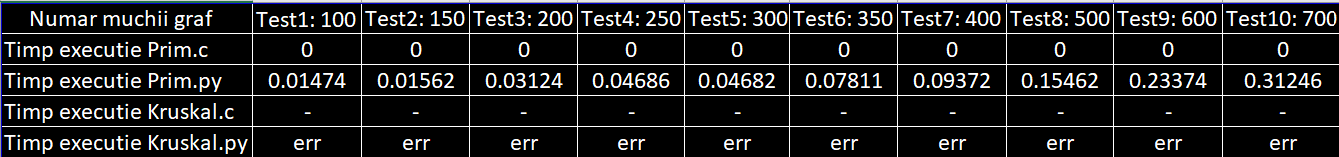
\includegraphics[width = 15cm, height = 3.5cm]{tabel}
\end{center}
\vspace{2mm}

Unele dintre rezultate fiind foarte apropiate ca dimensiune, au fost exprimate cu mai multe zecimale pentru a putea fi pus\u{a} \^in eviden\c t\u{a} evolu\c tia lor.\\
\vspace{1mm}
Rezultatele pot fi vizualizate \^in graficul ata\c sat mai jos.
\vspace{2mm}
\begin{center}
    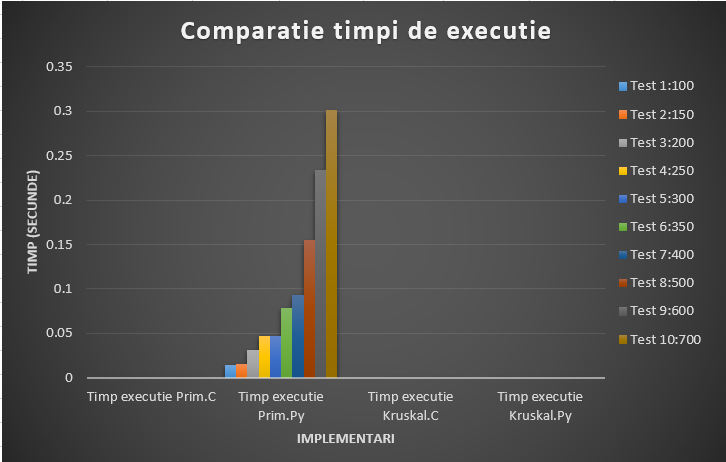
\includegraphics[width = 14cm, height = 10cm]{grafic3.0}
\end{center}
\begin{center}
    \colorbox{black}{\textcolor{white}{\textbf{-Grafic analiz\u{a} timpi de execu\c tie-}}}
\end{center}
%\textbf{-Grafic analiza timpi de executie-}

\vspace{4mm}
\^In cazul algoritmului lui Prim se poate observa ca ambele implementari, at\^at cea in limbajul C, c\^at si cea \^in limbajul Python sunt foarte eficiente pentru un numar relativ mare de muchii ale grafului.\\
   Totu\c si, se observ\u{a} o cre\c stere a timpului de execu\c tie \^in cazul implement\u{a}rii \^in limbajul Python fa\c t\u{a} de limbajul C, \^in ciuda faptului c\u{a} aceasta nu este una exponen\c tial\u{a} ( accentuat\u{a} ).Totu\c si, pentru aceste seturi de date, aceasta exist\u{a}.\\
Pentru implementarea \^in limbajul C, timpul de execu\c tie r\u{a}m\^ane aproximativ constant \c si infim (tinde c\u{a}tre 0 pentru toate seturile de date \^in acest caz).\\
Aceast\u{a} discrepan\c t\u{a} este motivat\u{a} de natura diferit\u{a} a celor dou\u{a} limbaje de programare.\\\underline{Limbajul C} este un limbaj compilat, ale c\u{a}rui intruc\c tiuni sunt convertite direct \^in cod ma\c sin\u{a} care poate fi executat de c\u{a}tre procesor.\^In consecin\c t\u{a}, limbajele de programare care se \^incadreaza \^in aceast\u{a} categorie tind sa fie mai rapide.\\
\^In cazul \underline{limbajului Python}, care se \^incadreza \^in categoria limbajelor de programare interpretate, fiecare instruc\c tiune este analizat\u{a}(interpretat\u{a}) \c si executat\u{a} pe r\^and la momentul respectiv.\\
\\
Mai multe referitor la acest topic:\\\\ -\textcolor{blue}{\url{https://www.freecodecamp.org/news/compiled-versus-interpreted-languages/}}\\ -\textcolor{blue}{\url{https://stackoverflow.com/questions/3265357/compiled-vs-interpreted-languages}}\\ 
-\textcolor{blue}{\url{https://www.geeksforgeeks.org/compiler-vs-interpreter-2/}}\\

\vspace{3mm}
\newline
De\c si \^in cazul algortimului lui Kruskal pentru aflarea arborelui de acoperire minim\u{a} nu s-au putut exprima \c si afi\c sa rezultate palpabile si concrete(implementarea realizat\u{a} este instabil\u{a}, neput\^and fii extrase rezultate conving\u{a}toare; algoritmul ruleaz\u{a}, ofer\u{a} informa\c tii, \^insa nu \c \c si timpul corect de formare al arborelui de acoperire minim\u{a}, astfel \^inc\^at analiza temporal\u{a} nu s-a putut realiza cu precizie), din analiza complexita\c tii celor doi algoritmi se poate deduce faptul c\u{a} este mai ineficient \^in compara\c tie direct\u{a} cu algoritmul lui Prim.\\
\\
De\c si este \^in continuare un algoritm eficient(din unele m\u{a}sur\u{a}tori aleatorii care s-au putut realiza), timpii de execu\c tie surprin\c si sunt mai mari dec\^at \^in cazul algoritmului lui Prim, fiind vorba de asemenea de valori foarte apropiate de valoarea 0 (inclusiv pentru un num\u{a}r semnificativ de muchii ale grafului).\\
Totu\c si, \c si acest aspect are mai multe unghiuri din care poate fi analizat.\\\\C\^and este vorba despre un graf dens, care are un num\u{a}r semnificativ mai mare de muchii (raportat la num\u{a}rul de noduri ale grafului), \^intotdeauna abordarea algoritmului lui Prim va avea rezultate mai bune. Pe de alt\u{a} parte, \^in cazul grafurilor "r\u{a}sfirate" (\underline{sparse}), cu un num\u{a}r relativ mic de muchii, algoritmul lui Kruskal este mai potrivit pentru formarea arborelui de acoperire minim\u{a}.\\
\\
\underline{\textbf{Men\c tiune:}} \^in cadrul acestui raport nu au fost abordate cele mai eficiente implement\u{a}ri ale celor doi algoritmi.Am realizat implement\u{a}rile utiliz\^and elemente cu care sunt familiarizat \c si cu care am fost capabil sa operez.Din documenta\c tia f\u{a}cut\u{a} pentru realizarea acestui proiect, am descoperit metode mai eficiente de implementare a acestor algoritmi, \^ins\u{a} acestea implicau no\c tiuni necunoscute mie, dar care pot deveni subiect de studiu \^in viitorul apropiat.
\\\\\\
-\underline{\textbf{Concluzii \& g\^anduri personale} referitoare la proiectul realizat}-\\

Dup\u{a} timp \c si resurse investite, am putut livra toate componentele necesare asign\u{a}rii acestui proiect(\^in m\u{a}sura \^in care am fost capabil \c si \^in forma prezentat\u{a}), ceea ce m\u{a} bucur\u{a} \^intr-o anumit\u{a} m\u{a}sur\u{a}, dar pe de alt\u{a} parte, am descoperit c\^at de mult mai am de acumulat(\c si de \^insu\c sit cuno\c stin\c te de asemenea) \c si c\^at de vast este acest univers, dac\u{a} m\u{a} pot exprima astfel.\\\\
Am \^int\^ampinat dificult\u{a}\c ti \^in ceea ce prive\c ste implementarea algoritmilor \^in limbajul Python, necunoscut mie si neav\^and experien\c t\u{a} \^in utilizarea acestuia.O consecin\c t\u{a} a acestui fapt este ca nu am putut livra o versiune executabil\u{a} a algoritmului lui Kruskal \^in limbajul Python.Nu mi-am putut \^insusi anumite aspecte \c si particularit\u{a}\c ti referitoare la acest limbaj \^in timpul acordat finaliz\u{a}rii produselor livrabile(spre exemplu, substituirea structurilor din limbajul C, care de altfel, am \^inteles ca nu sunt disponibile \^intr-un format similar \^in limbajul Python).\\\\
Un alt inconvenient a fost crearea si utilizarea fi\c sierelor Makefiles.Am \^incercat sa le implementez pentru generatorul de date(structura \c si logica cred ca sunt corecte), \^ins\u{a} am \^int\^ampinat dificulta\c ti la navigarea prin sistemul de operare utiliz\^and bash-ul.Am utilizat pachetul Linux pus la dispozi\c tie de Windows 10.\\\\
Pe de alt\u{a} parte, acest proiect pot spune c\u{a} m-a responsabilizat \c si prin intermediul lui am experimentat lucruri noi si am luat contact cu tehnologii diverse, cu unele dintre acestea fiind la primul contact.\\\\
\^In viitorul apropiat doresc s\u{a} aprofundez dezvoltarea programelor \^in limbajul Python; de asemenea, editorul de text Latex reprezint\u{a} din nou un punct de atrac\c tie si de curiozitate pentru mine. Este un tool util si intuitiv ( am descoperit asta dup\u{a} ce m-am acomodat cu el). Realizarea \c si prelucrarea raportului de lucru utiliz\u{a}nd Latex a devenit un lucru pl\u{a}cut pentru mine, fiind atras si "pasionat" de formatare si editare.\\\\
Un alt aspect important care consider c\u{a} merit\u{a} amintit este impunerea termenului limit\u{a} care a trebuit respectat.Consider ca acest parametru a condus la o organizare \c si la o coordonare mai bun\u{a} a timpului si a celorlalte aspecte implicate \^in realizarea temei de cas\u{a} \^in ansamblu, ceea ce constituie de asemenea cerin\c te \c si criterii pe care un viitor activant \^in domeniul tehnologiei trebuie s\u{a} \c si le \^insu\c seasc\u{a}.
\\
\\

\subsection{Referin\c te}

\begin{thebibliography}{10}

	\bibitem{cormen}
	 Thomas H. Cormen and Charles E. Leiserson and Ronald L. Rivest and Clifford Stein,
	  \emph{Introduction to Algorithms}.
	  MIT Press,
	  3rd Edition,
	  2009.
	
	\bibitem{latex}
     \LaTeX~project site,
     \textcolor{blue}{\url{http://latex-project.org/}}
     
     \bibitem{overleaf}
       \LaTeX~documentation site,
     \textcolor{blue}{\url{https://www.overleaf.com/learn}}
     
     \bibitem{latex book}
     \textbf{INTRODUCERE \^IN LIMBAJUL LATEX},
      \textcolor{blue}{\url{https://docs.google.com/viewer?a=v&pid=sites&srcid=ZGVmYXVsdGRvbWFpbnx1Y3Z0cGxhYnxneDoyNDBmN2UyZGNmZDhhNjU3}}

\bibitem{stackoverflow}
StackOverflow: \textcolor{blue}{\url{https://stackoverflow.com/}}

\bibitem{wikipedia}
Wikipedia: \textcolor{blue}{\url{https://www.wikipedia.org/}}

\bibitem{quora}
Quora : \textcolor{blue}{\url{https://www.quora.com/}}

\bibitem{geekforgeeks}
GeekForGeeks : \textcolor{blue}{\url{https://www.geeksforgeeks.org/}} 

\bibitem{includehelp}
IncludeHelp :\textcolor{blue}{ \url{https://www.includehelp.com/c-programming-questions/what-is-makefile.aspx}}

\bibitem{youtube}
YouTube : \textcolor{blue}{\url{https://www.youtube.com/}}
\end{thebibliography}
\\


\underline{\textbf{\textcolor{red}{Not\u{a}:}}} unele dintre referin\c te sunt men\c tionate \c si \^in con\c tinutul raportului \^inso\c tite de alte preciz\u{a}ri.

\end{document}








